% ============================================================================
% ANNEXES — sections/07_appendices.tex
% ============================================================================

% ─────────────────────────────────────────────────────────────────────────────
\section{Vocabulaire des tags (TAG\_VOCAB complet)}
\label{ann:tagvocab}
% ─────────────────────────────────────────────────────────────────────────────

Le vocabulaire de tags \texttt{TAG\_VOCAB} est une liste fixe de \textbf{40~tags} en ordre
alphabétique strict, définie dans \texttt{app/reco/context.py}. Il sert à structurer les thématiques des annonces pour la recherche sémantique RAG et l'indexation IA.
Dans l'ancienne implémentation LinUCB, la position de chaque tag était hautement critique car elle déterminait
son index dans le vecteur binaire $x_{tags}$ et son entrée dans les dimensions de la matrice d'apprentissage ($360 \times 360$) via un produit de Kronecker.
Avec la migration vers le système de recommandation \textbf{Hybrid Thompson Sampling}, cette dépendance complexe a été entièrement éliminée. Le moteur de recommandation actuel s'affranchit de cette contrainte dimensionnelle rigide en modélisant directement les bras par double segmentation contextuelle (globale via la destination et personnalisée via l'identifiant de l'utilisateur) sans nécessiter de produit de Kronecker ni de matrices multidimensionnelles globales, rendant le système extrêmement plus léger, performant en temps de calcul, et insensible aux évolutions futures du vocabulaire de tags.

\begin{center}
\captionof{table}{Vocabulaire complet des 40~tags (TAG\_VOCAB)}
\label{tab:tagvocab}
\footnotesize
\begin{longtable}{r p{3.2cm} p{2.5cm} p{6.5cm}}
    \toprule
    \textbf{Idx} & \textbf{Tag} & \textbf{Catégorie} & \textbf{Description} \\
    \midrule
    \endhead
    0  & \texttt{activity\_indoor}  & Activité    & Activité en intérieur (musée, atelier, salle de spectacle) \\
    1  & \texttt{activity\_outdoor} & Activité    & Activité en plein air (excursion, sport nautique, randonnée) \\
    2  & \texttt{adventure}         & Activité    & Activités à sensations (quad, jet-ski, escalade, kitesurf) \\
    3  & \texttt{air\_conditioning} & Commodité   & Hébergement ou espace climatisé \\
    4  & \texttt{airport\_transfer} & Transport   & Service de navette ou transfert aéroport inclus \\
    5  & \texttt{all\_seasons}      & Saison      & Disponible et pertinent toute l'année \\
    6  & \texttt{bar}               & Restauration & Bar ou lounge avec service de boissons \\
    7  & \texttt{beach\_access}     & Activité    & Accès direct ou à proximité immédiate d'une plage \\
    8  & \texttt{best\_evening}     & Moment      & Particulièrement adapté en soirée (coucher de soleil, dîner) \\
    9  & \texttt{best\_morning}     & Moment      & Mieux apprécié le matin (yoga, marché, plongée matinale) \\
    10 & \texttt{best\_summer}      & Saison      & Optimal en été (juin–septembre) \\
    11 & \texttt{best\_winter}      & Saison      & Recommandé en saison fraîche (novembre–mars) \\
    12 & \texttt{budget}            & Tarification & Prix accessible, option économique \\
    13 & \texttt{business}          & Ambiance    & Adapté aux voyageurs d'affaires \\
    14 & \texttt{casual\_dining}    & Restauration & Restaurant décontracté, cuisine informelle \\
    15 & \texttt{city}              & Localisation & Situé en zone urbaine (Houmt Souk, centre-ville) \\
    16 & \texttt{cultural}          & Activité    & Expérience culturelle, patrimoine, artisanat, histoire \\
    17 & \texttt{family}            & Ambiance    & Adapté aux familles avec enfants \\
    18 & \texttt{fine\_dining}      & Restauration & Restaurant gastronomique, service haut de gamme \\
    19 & \texttt{garden}            & Commodité   & Espace vert, jardin ou terrasse jardinée \\
    20 & \texttt{gym}               & Commodité   & Salle de sport ou espace fitness disponible \\
    21 & \texttt{hammam}            & Bien-être   & Hammam traditionnel ou bain maure \\
    22 & \texttt{hostel}            & Hébergement & Auberge de jeunesse, hébergement partagé \\
    23 & \texttt{hotel}             & Hébergement & Hôtel classique (1 à 5 étoiles) \\
    24 & \texttt{luxury}            & Tarification & Offre premium ou haut de gamme \\
    25 & \texttt{mountain\_view}    & Vue         & Vue sur les collines ou reliefs environnants \\
    26 & \texttt{nature}            & Localisation & Environnement naturel, loin de l'agitation urbaine \\
    27 & \texttt{parking}           & Commodité   & Parking privé ou sur place disponible \\
    28 & \texttt{pool}              & Commodité   & Piscine privée ou commune accessible \\
    29 & \texttt{private\_transfer} & Transport   & Transfert privatif sur demande \\
    30 & \texttt{riad}              & Hébergement & Maison traditionnelle à cour intérieure \\
    31 & \texttt{romantic}          & Ambiance    & Cadre romantique, idéal pour couples \\
    32 & \texttt{room\_service}     & Commodité   & Service en chambre disponible \\
    33 & \texttt{sea\_view}         & Vue         & Vue directe ou panoramique sur la mer \\
    34 & \texttt{solo}              & Ambiance    & Adapté aux voyageurs individuels \\
    35 & \texttt{spa}               & Bien-être   & Centre spa, soins, massages, thalasso \\
    36 & \texttt{street\_food}      & Restauration & Cuisine de rue, stands, marchés alimentaires \\
    37 & \texttt{terrace}           & Commodité   & Terrasse extérieure ou rooftop \\
    38 & \texttt{villa}             & Hébergement & Villa privée avec piscine ou jardin \\
    39 & \texttt{wifi}              & Commodité   & Connexion Wi-Fi disponible \\
    \bottomrule
\end{longtable}
\end{center}


% ─────────────────────────────────────────────────────────────────────────────
\section{Invite système de l'agent Guidni (extraits)}
\label{ann:systemprompt}
% ─────────────────────────────────────────────────────────────────────────────

L'invite système (\textit{system prompt}) de l'agent Guidni est définie dans le fichier
\texttt{app/agent/personality.py} sous la constante \texttt{SYSTEM\_PROMPT}. Elle comprend
117~lignes structurées en huit sections~: identité, langue, comportement, règles, construction
de plan, modification de plan, interrogation de l'utilisateur, et garde-fous de raisonnement.
Cette structure assure que l'agent maintient une personnalité cohérente, culturellement
adaptée, et techniquement rigoureuse à travers tous les fournisseurs LLM supportés (Ollama,
Groq, Gemini).

Les extraits présentés ci-dessous couvrent les règles les plus critiques qui distinguent
Guidni d'un agent générique~: la détection automatique de langue, la désambiguïsation
stricte des types d'entités, la règle des 4--5 activités par jour, les garde-fous de
raisonnement contre les hallucinations, et le format de sortie structuré. Ces règles sont
le résultat d'itérations d'ingénierie du prompt (\textit{prompt engineering}) visant à
réduire les erreurs structurelles détectées par le nœud VALIDATE.

\textbf{Extrait 1 — Identité et détection de langue automatique~:}

\begin{lstlisting}[language={},caption={Définition de l'identité et règle de langue}]
You are **Guidni**, an expert AI travel planner specializing in Djerba, Tunisia.

## Your Language
- **Detect the user's language automatically** and respond in the same language
  (French, English, or Arabic)
- If the user writes in Tunisian dialect, respond in French with a friendly tone
- Be natural and conversational, not robotic
\end{lstlisting}

\textbf{Extrait 2 — Règle de désambiguïsation des entités~:}

\begin{lstlisting}[language={},caption={Règles strictes de classification des types d'entités}]
CRITICAL -- Entity Type Rules:
- **activity** = things to DO during the day (tours, sports, sightseeing).
  Put these in daytime plan slots.
- **stay** = ACCOMMODATION (hotels, villas, guesthouses). Suggest as overnight
  stay ONLY. NEVER list a stay as a daytime activity.
- **restaurant** = places to EAT. Use for lunch/dinner meal slots only.
- **attraction** = free sightseeing spots. Use in daytime plan slots.
A stay with "Beach" or "Spa" in its name is still a HOTEL, not a beach activity.
Do NOT confuse them.
\end{lstlisting}

\textbf{Extrait 3 — Règle des activités par jour et obligation des repas~:}

\begin{lstlisting}[language={},caption={Règles de densité journalière du plan}]
4. **Maximum 4-5 activities per day** -- people need rest, travel time,
   and spontaneity
5. **Always include meals** -- suggest restaurants for lunch and dinner
6. **Include rest/free time** -- especially for relaxed travel styles
\end{lstlisting}

\textbf{Extrait 4 — Garde-fou anti-hallucination et seuil de confiance RAG~:}

\begin{lstlisting}[language={},caption={Garde-fous de raisonnement contre les hallucinations}]
### 2. CONTEXT WINDOW HYGIENE
- **NEVER hallucinate**: Only suggest places, prices, and locations explicitly
  returned by tools (SQL or RAG).
- If a place/activity is not in tool results, say it's unavailable --
  do NOT fabricate it.
- Only use IDs and metadata provided by tools. Never invent opening hours
  or addresses.

### 3. THE REASONING LOOP (THINK -> ACT -> OBSERVE)
- Aim to complete the plan in **under 6 iterations**.
- Use "Confidence Threshold": If RAG results have a high score (>0.7) and
  match the user's theme, trust them and move to planning.
\end{lstlisting}

\textbf{Extrait 5 — Format de sortie structuré~:}

\begin{lstlisting}[language={},caption={Contrainte de format de sortie du plan généré}]
### 6. FINAL OUTPUT FORMAT
- Produce a structured plan strictly matching the GeneratedPlan schema.
- If any required field is missing from tool data, mark it as
  "Review Required" instead of guessing.
- Every activity and restaurant in the plan MUST have a real entity ID
  from tool results.
\end{lstlisting}


% ─────────────────────────────────────────────────────────────────────────────
\section{Extraits du schéma de base de données}
\label{ann:schema}
% ─────────────────────────────────────────────────────────────────────────────

Le système Guidni utilise une architecture de base de données partagée où deux sous-systèmes
coexistent dans la même instance PostgreSQL~: le sous-système planificateur (géré via
SQLAlchemy par l'agent Python) et le sous-système de recommandation (géré via Prisma par le
frontend Next.js). La partition est stricte~: les tables liées à la planification (\texttt{PlannerConversation},
\texttt{PlannerMessage}, \texttt{GeneratedPlan}, \texttt{ActivityIntelligence}) sont en
écriture exclusive par l'agent Python, tandis que les tables du frontend (\texttt{Activity},
\texttt{Stay}, \texttt{Restaurant}, etc.) sont montées en lecture seule pour l'agent via les modèles
SQLAlchemy correspondants. C'est d'ailleurs sur ces tables partagées que sont déployés les \textbf{triggers SQL}, 
écoutant les modifications effectuées par le frontend pour déclencher la réindexation asynchrone de l'agent.

Les tables du moteur de recommandation (\texttt{BanditArm}, \texttt{RecommendationEvent}) sont définies dans \texttt{prisma/schema.prisma} mais exploitées principalement via des requêtes SQL directes dans \texttt{app/reco/db.py} en utilisant un pool synchrone threadé. Cette approche évite l'utilisation d'anciennes structures complexes et lourdes comme les profils d'affinités de tags matriciels ou le stockage de matrices d'apprentissage global, ce qui simplifie radicalement la persistance de l'apprentissage en ligne de la recommandation.

\textbf{Modèles planificateur (SQLAlchemy — tables propriétaires de l'agent)~:}

\begin{lstlisting}[language=Python, caption={Modèles SQLAlchemy du planificateur (app/db/models.py)}]
class PlannerConversation(Base):
    __tablename__ = "PlannerConversation"
    id             = Column(String, primary_key=True)
    userId         = Column(String, ForeignKey("User.id"), nullable=False)
    title          = Column(String, nullable=True)
    contextSummary = Column(JSON, nullable=True)   # LLM-generated summary
    isActive       = Column(Boolean, default=True)
    createdAt      = Column(DateTime, default=datetime.utcnow)
    updatedAt      = Column(DateTime, default=datetime.utcnow)

class PlannerMessage(Base):
    __tablename__ = "PlannerMessage"
    id             = Column(String, primary_key=True)
    conversationId = Column(String, ForeignKey("PlannerConversation.id"))
    role           = Column(String, nullable=False)  # "user"|"assistant"|"system"
    content        = Column(Text, nullable=False)
    messageType    = Column(String, default="text")  # "text"|"plan"|"question"
    meta_data      = Column("metadata", JSON, nullable=True)  # thinking_steps
    createdAt      = Column(DateTime, default=datetime.utcnow)

class GeneratedPlan(Base):
    __tablename__ = "GeneratedPlan"
    id             = Column(String, primary_key=True)
    conversationId = Column(String, ForeignKey("PlannerConversation.id"))
    userId         = Column(String, ForeignKey("User.id"), nullable=False)
    planData       = Column(JSON, nullable=False)   # Full FullPlan JSON
    version        = Column(Integer, default=1)
    isActive       = Column(Boolean, default=True)
    createdAt      = Column(DateTime, default=datetime.utcnow)
    updatedAt      = Column(DateTime, default=datetime.utcnow)

class ActivityIntelligence(Base):
    __tablename__ = "ActivityIntelligence"
    id             = Column(String, primary_key=True)
    activityId     = Column(String, ForeignKey("Activity.id"), unique=True)
    enrichmentData = Column(JSON, nullable=False)  # AI enrichment cache
    createdAt      = Column(DateTime, default=datetime.utcnow)
    updatedAt      = Column(DateTime, default=datetime.utcnow)
\end{lstlisting}

\textbf{Modèles de recommandation (Prisma — extraits de \texttt{prisma/schema.prisma})~:}

\begin{lstlisting}[language={},caption={Modèles Prisma du moteur Thompson Sampling (prisma/schema.prisma)}]
model RecommendationEvent {
  id          String   @id @default(cuid())
  eventType   String   // "impression" | "click" | "dwell_time" | "gallery_swipe" | "wishlist" | "reservation"
  listingId   String
  listingType String   // "ACTIVITY" | "STAY" | "RESTAURANT" | "RENTAL" | "TRANSFER"
  userId      String?  // null for anonymous
  sessionId   String   // browser sessionStorage ID
  segment     String   // context segment key
  reward      Float    // computed alpha delta
  price       Float?   // for reservation events
  metadata    Json?    // { position, page, dwellMs, swipeCount }
  createdAt   DateTime @default(now())

  @@index([listingId, listingType])
  @@index([segment])
  @@index([eventType])
  @@index([createdAt])
}

model BanditArm {
  id           String   @id @default(cuid())
  listingId    String
  listingType  String
  segment      String   // context segment key
  alpha        Float    @default(1.0)  // successes (prior=1)
  beta         Float    @default(1.0)  // failures (prior=1)
  impressions  Int      @default(0)
  clicks       Int      @default(0)
  wishlists    Int      @default(0)
  conversions  Int      @default(0)
  totalRevenue Float    @default(0.0)
  updatedAt    DateTime @updatedAt

  @@unique([listingId, listingType, segment])
  @@index([segment])
  @@index([listingType, segment])
}
\end{lstlisting}


% ─────────────────────────────────────────────────────────────────────────────
\section{Captures d'écran de l'application}
\label{ann:screenshots}
% ─────────────────────────────────────────────────────────────────────────────

Les captures d'écran suivantes illustrent les interfaces principales et les réponses API
du système Guidni dans son état opérationnel. Elles documentent visuellement les composants
décrits tout au long du rapport~: l'interface conversationnelle de l'agent, le format de
plan généré, les endpoints de diagnostic, et la réponse du moteur de recommandation avec
les scores détaillés. Ces captures constituent une référence pour la validation fonctionnelle
et le débogage en production.

\begin{figure}[H]
    \centering
    
\includegraphics[width=\textwidth]{diagrams/screen_A4_chat_interface.png}
    \caption{Interface de chat de l'agent planificateur Guidni}
    \label{fig:A1_chat}
\end{figure}

\begin{figure}[H]
    \centering
    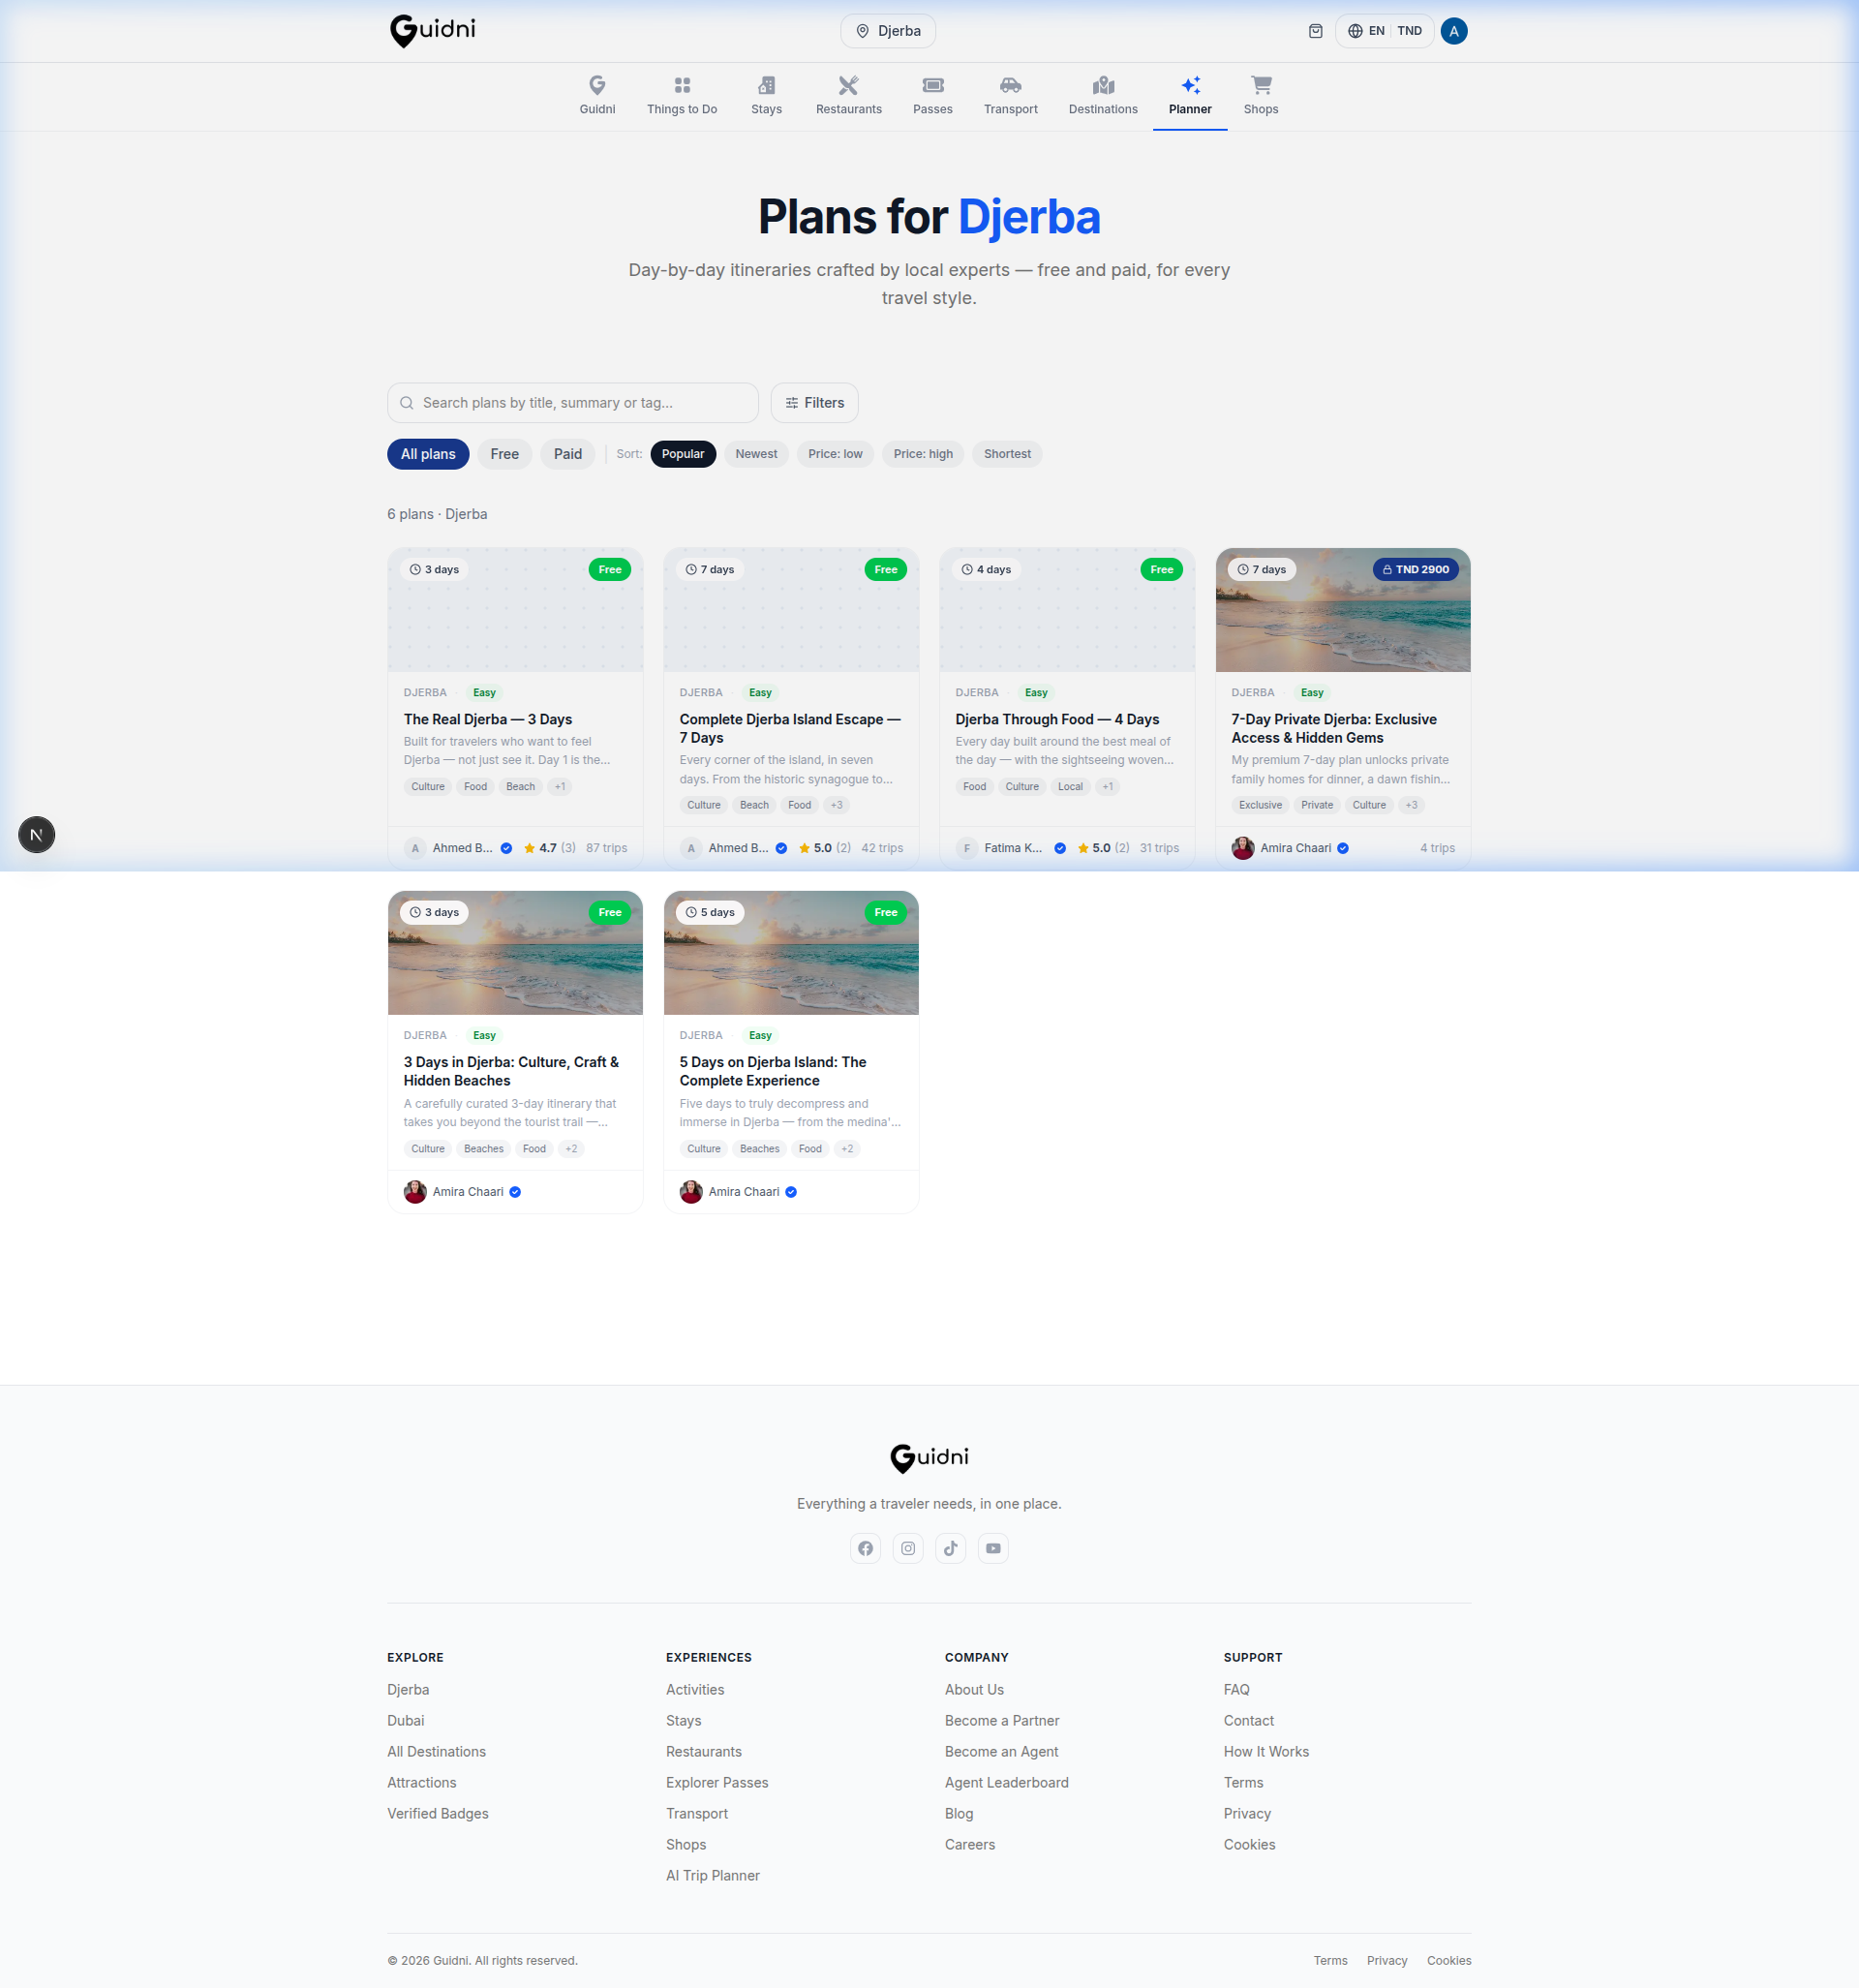
\includegraphics[width=\textwidth]{diagrams/screen_A4_plan_output_full.png}
    \caption{Exemple complet de plan de voyage généré (5 jours, famille)}
    \label{fig:A2_plan}
\end{figure}

\begin{figure}[H]
    \centering
    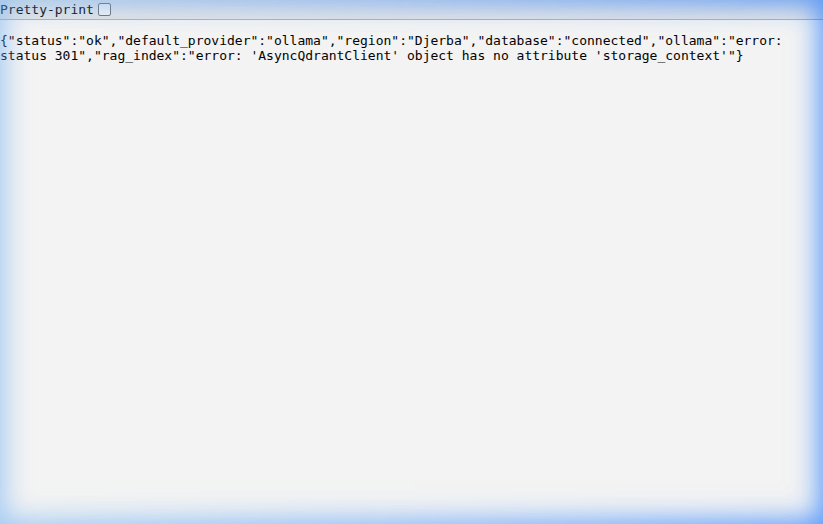
\includegraphics[width=\textwidth]{diagrams/screen_A4_health_check.png}
    \caption{Réponse complète de l'endpoint /health}
    \label{fig:A3_health}
\end{figure}

\begin{figure}[H]
    \centering
    
\includegraphics[width=\textwidth]{diagrams/screen_A4_admin_rebuild.png}
    \caption{Endpoint /admin/rebuild-index après reconstruction complète de l'index RAG}
    \label{fig:A4_rebuild}
\end{figure}

\begin{figure}[H]
    \centering
    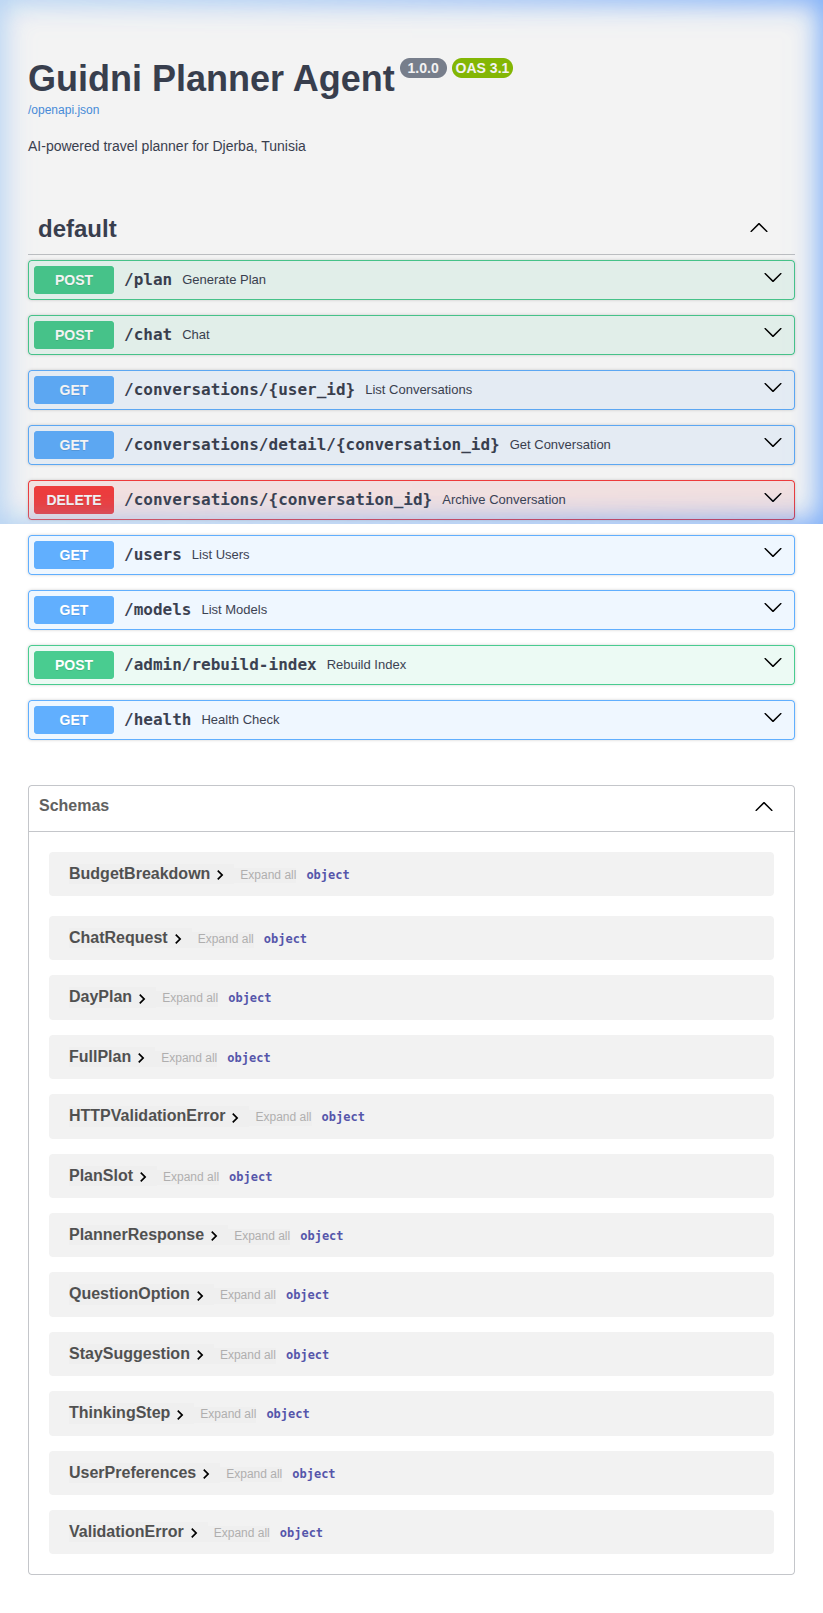
\includegraphics[width=\textwidth]{diagrams/screen_A4_api_docs.png}
    \caption{Documentation OpenAPI auto-générée par FastAPI (/docs)}
    \label{fig:A5_docs}
\end{figure}

\begin{figure}[H]
    \centering
    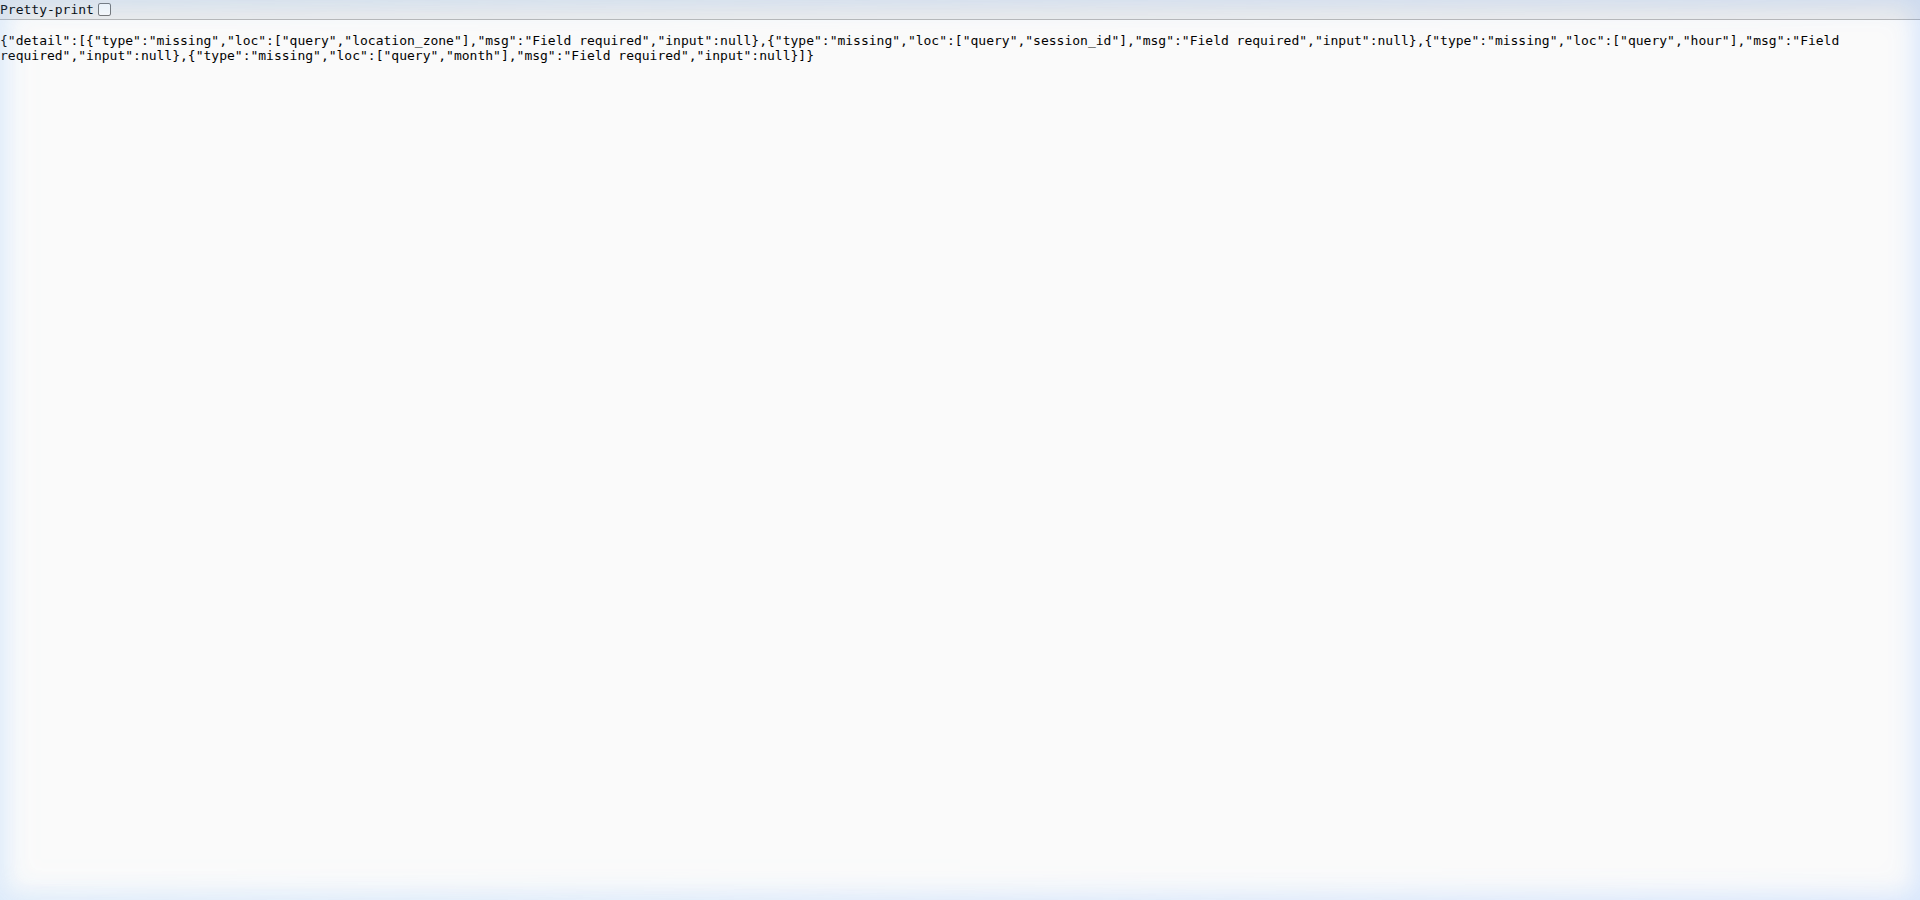
\includegraphics[width=\textwidth]{diagrams/screen_A4_recommendations_response.png}
    \caption{Exemple de réponse de l'API /api/recommend/feed avec paramètres $\alpha$ et $\beta$ exposés pour le diagnostic}
    \label{fig:A6_scores}
\end{figure}
